% ------------------------------------------------------------------------------
% TYPO3 CMS 7.3 - What's New (English Version)
%
% @author	Michael Schams <schams.net>
% @license	Creative Commons BY-NC-SA 3.0
% @link		http://typo3.org/download/release-notes/whats-new/
% @language	English
% ------------------------------------------------------------------------------
% LTXE-CHAPTER-UID:		cc6b358d-f0ed36d3-f7a72fa2-af63ccfc
% LTXE-CHAPTER-NAME:	Backend User Interface
% ------------------------------------------------------------------------------

\section{Backend / Внутренний интерфейс}
\begin{frame}[fragile]
	\frametitle{Backend / Внутренний интерфейс}

	\begin{center}\huge{Глава 1:}\end{center}
	\begin{center}\huge{\color{typo3darkgrey}\textbf{Backend / Внутренний интерфейс}}\end{center}

\end{frame}

% ------------------------------------------------------------------------------
% LTXE-SLIDE-START
% LTXE-SLIDE-UID:		fcf9e90b-9a774854-3c20ede7-e0974d81
% LTXE-SLIDE-ORIGIN:	111332b8-ac46a07a-319ed582-f873bc02 English
% LTXE-SLIDE-ORIGIN:	b4dc1576-57b4854f-26a32d85-11f7c52b German
% LTXE-SLIDE-TITLE:		Feature #66173: Allow page title edit by doubleclick
% LTXE-SLIDE-REFERENCE:	Feature-66173-AllowPageTitleEditByDoubleclick.rst
% ------------------------------------------------------------------------------
\begin{frame}[fragile]
	\frametitle{Backend / Внутренний интерфейс}
	\framesubtitle{Название страницы в модулях Страница и Список}

	Изменить названия страниц в модулях "Страница" и "Список" теперь можно дважды щёлкнув
	по заголовку страницы или по значку редактирования.

	\begin{figure}
		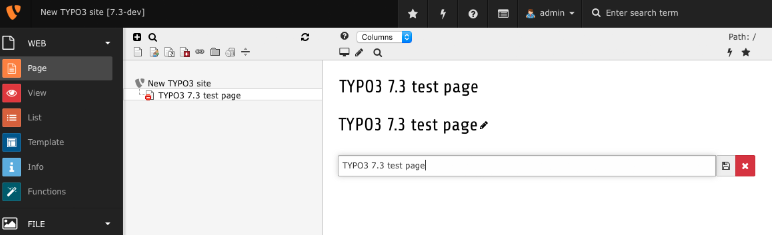
\includegraphics[width=0.9\linewidth]{BackendUserInterface/66173.png}
	\end{figure}

\end{frame}

% ------------------------------------------------------------------------------
% LTXE-SLIDE-START
% LTXE-SLIDE-UID:		6786d08c-2079149e-a804dd75-c4d6d49c
% LTXE-SLIDE-ORIGIN:	c17b263e-12512d4b-13d5389f-df1ec14e English
% LTXE-SLIDE-ORIGIN:	168b1424-1ebb2552-ed5bac3e-8a9ac737 German
% LTXE-SLIDE-TITLE:		Feature #67071: Processed files cleanup tool added in Install Tool
% LTXE-SLIDE-REFERENCE:	Feature-67071-ProcessedFilesCleanupToolAddedInInstallTool.rst
% ------------------------------------------------------------------------------
\begin{frame}[fragile]
	\frametitle{Backend / Внутренний интерфейс}
	\framesubtitle{Install Tool: удаление обработанных файлов}

	В разделе "Clean up" из Install Tool добавлен новый функционал для удаления
	временных файлов (например, эскизов изображений) из FAL.\newline
	Это полезно при изменении настроек для работы с графикой, либо после обновления
	GraphicsMagick/ImageMagick для принудительного пересоздания всех изображений.

	\begin{figure}
		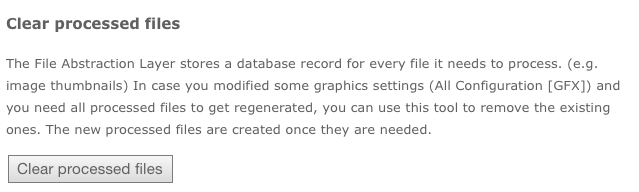
\includegraphics[width=0.6\linewidth]{BackendUserInterface/67071.png}
	\end{figure}

\end{frame}

% ------------------------------------------------------------------------------
% LTXE-SLIDE-START
% LTXE-SLIDE-UID:		d43a15d5-5866b6d2-f9ba5e9f-9e441cb4
% LTXE-SLIDE-ORIGIN:	4662a0fc-e8a91f22-2f75e0bc-800e9b63 English
% LTXE-SLIDE-ORIGIN:	daa83c1e-08d2716b-de74cbda-42361551 German
% LTXE-SLIDE-TITLE:		Feature #67319: Add field "copyright" to EXT:filemetadata
% LTXE-SLIDE-REFERENCE:	Feature-67319-AddFieldCopyrightToEXTfilemetadata.rst
% ------------------------------------------------------------------------------
\begin{frame}[fragile]
	\frametitle{Backend / Внутренний интерфейс}
	\framesubtitle{Новое поле в мета данных FAL Meta Data}

	К мета данным записей FAL было добавлено поле "\textbf{Copyright}"
	(system extension: \texttt{filemetadata}).

	\begin{figure}
		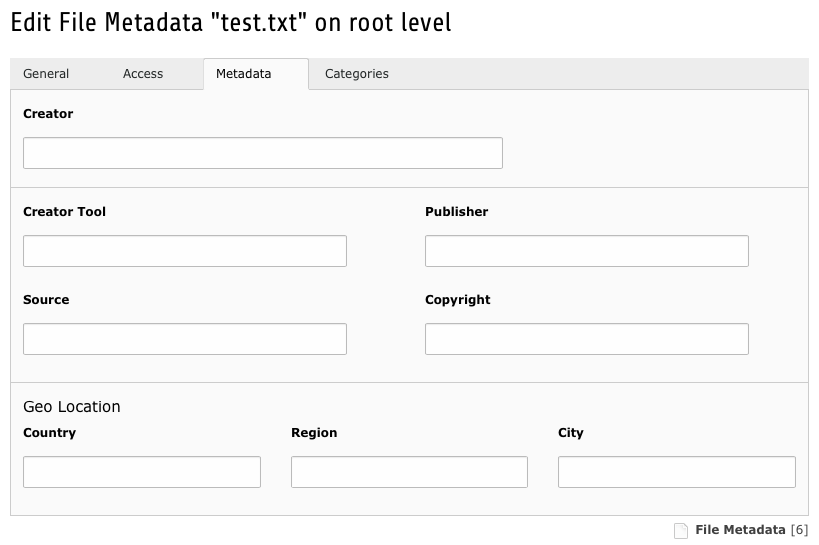
\includegraphics[width=0.6\linewidth]{BackendUserInterface/67319.png}
	\end{figure}

\end{frame}

% ------------------------------------------------------------------------------
